% ============================================================
% INTRODUCTION ET VUE D'ENSEMBLE
% ============================================================
\chapter{Introduction}

\section{Contexte et Motivation}

La Langue des Signes Française (LSF) est le principal moyen de communication pour environ 300\,000 personnes sourdes et malentendantes en France. Malgré sa richesse linguistique, la LSF reste largement incomprise par la majorité de la population entendante, créant une barrière de communication significative dans la vie quotidienne, professionnelle et sociale des personnes sourdes.

Les avancées récentes en vision par ordinateur et en intelligence artificielle offrent une opportunité unique de développer des outils de traduction automatique capables de reconnaître les gestes de la LSF en temps réel et de les convertir en texte ou en parole. Ce projet s'inscrit dans cette démarche en proposant un système complet de traduction de la LSF, fonctionnant localement sur un PC standard équipé d'une webcam, ainsi que sur un Raspberry Pi 4B pour un déploiement embarqué et portable.

\section{Objectifs du Projet}

Les objectifs principaux de ce projet sont :

\begin{itemize}
    \item \textbf{Reconnaissance en temps réel} : Développer un pipeline capable de détecter et classifier les signes statiques (lettres et chiffres) de la LSF à partir d'un flux vidéo en direct.
    \item \textbf{Architecture modulaire} : Concevoir une architecture en pipeline composée de modules indépendants et réutilisables (acquisition, estimation de pose, ingénierie des caractéristiques, classification, interface).
    \item \textbf{Optimisation matérielle} : Exploiter le multithreading, la quantification des modèles et l'accélération GPU pour garantir des performances temps réel.
    \item \textbf{Déploiement embarqué} : Porter le système sur Raspberry Pi 4B avec caméra Pi v2.1 pour un usage portable et autonome.
    \item \textbf{Accessibilité} : Intégrer une synthèse vocale (TTS), un flux vidéo MJPEG accessible via navigateur, et un système de publication MQTT pour l'interopérabilité IoT.
\end{itemize}

\section{Architecture Générale}

Le système suit une architecture en pipeline modulaire composée de cinq modules principaux :

\begin{enumerate}
    \item \textbf{Module 1 -- Acquisition} : Capture vidéo threadée avec buffer circulaire et détection de mouvement MOG2.
    \item \textbf{Module 2 -- Estimation de Pose} : Extraction des 21 landmarks 3D de la main via MediaPipe Hands.
    \item \textbf{Module 3 -- Ingénierie des Caractéristiques} : Calcul de 15 angles articulaires, 63 coordonnées normalisées, et fenêtre temporelle adaptative.
    \item \textbf{Module 4 -- Classification} : Modèle MobileNetV3-Small pour les signes statiques, LSTM/GRU/Transformer pour les signes dynamiques.
    \item \textbf{Module 5 -- Interface d'Accessibilité} : Synthèse vocale, flux MJPEG Flask, et publication MQTT.
\end{enumerate}

\begin{figure}[H]
    \centering
    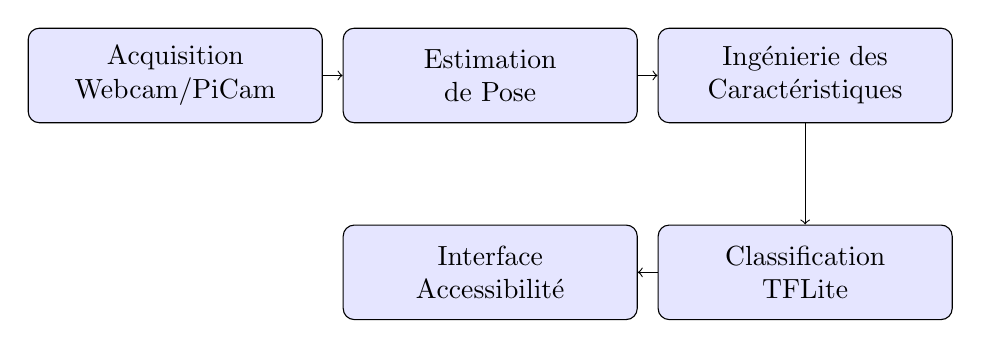
\begin{tikzpicture}[node distance=2.5cm, auto,
        block/.style={rectangle, draw, fill=blue!10, text width=3.5cm, text centered, rounded corners, minimum height=1.2cm}]
        \node[block] (acq) {Acquisition\\Webcam/PiCam};
        \node[block, right of=acq, node distance=4cm] (pose) {Estimation\\de Pose};
        \node[block, right of=pose, node distance=4cm] (feat) {Ingénierie des\\Caractéristiques};
        \node[block, below of=feat, node distance=2.5cm] (clf) {Classification\\TFLite};
        \node[block, left of=clf, node distance=4cm] (out) {Interface\\Accessibilité};
        \draw[->] (acq) -- (pose);
        \draw[->] (pose) -- (feat);
        \draw[->] (feat) -- (clf);
        \draw[->] (clf) -- (out);
    \end{tikzpicture}
    \caption{Architecture en pipeline du traducteur LSF}
\end{figure}

\section{Technologies Utilisées}

\begin{table}[H]
    \centering
    \begin{tabular}{ll}
        \toprule
        \textbf{Composant} & \textbf{Technologie} \\
        \midrule
        Capture vidéo & OpenCV / Picamera2 \\
        Détection de main & MediaPipe Hands / TFLite \\
        Modèle statique & MobileNetV3-Small (TFLite) \\
        Modèle dynamique & LSTM / GRU / Transformer \\
        Quantification & INT8, FP16, FP32 \\
        Synthèse vocale & pyttsx3 (espeak-ng) \\
        Streaming & Flask (MJPEG) \\
        IoT & MQTT (Mosquitto) \\
        Matériel embarqué & Raspberry Pi 4B + Camera v2.1 \\
        \bottomrule
    \end{tabular}
    \caption{Stack technologique du projet}
\end{table}
